% tags: [pythagoras-theorem] [ford-circles]

\documentclass[12pt]{article}
%Gummi|065|=)
\usepackage{amsmath, amsfonts, amssymb}
\usepackage[margin=0.5in]{geometry}
\usepackage{xcolor}
\usepackage{graphicx}

%\usepackage{pifont}
\usepackage{amsmath}



\newcommand{\off}[1]{}
\DeclareMathSizes{20}{30}{20}{18}

\newcommand{\two }{\sqrt[3]{2}}
\newcommand{\four}{\sqrt[3]{4}}
\newcommand{\red}{\begin{tikz}[scale=0.25]
\draw[fill=red, color=red] (0,0)--(1,0)--(1,1)--(0,1)--cycle;\end{tikz}}
\newcommand{\blue}{\begin{tikz}[scale=0.25]
\draw[fill=blue, color=blue] (0,0)--(1,0)--(1,1)--(0,1)--cycle;\end{tikz}}
\newcommand{\green}{\begin{tikz}[scale=0.25]
\draw[fill=green, color=green] (0,0)--(1,0)--(1,1)--(0,1)--cycle;\end{tikz}}

\newcommand{\sq}[3]{\draw[#3] (#1,#2)--(#1+1,#2)--(#1+1,#2+1)--(#1,#2+1)--cycle;}

\usepackage{tikz}
\usetikzlibrary{decorations.markings}

\newcommand{\susy}{{\bf Q}}
\newcommand{\RV}{{\text{R}_\text{V}}}

\title{Scratchwork: Farey Fractions}
\date{}
\begin{document}

%\fontfamily{qag}\selectfont \fontsize{12.5}{15}\selectfont

\sffamily

\maketitle

\noindent Here's a nice question about Farey Fractions:

\newpage

\includegraphics[width=6in]{fractions-01.png} 

\newpage

\noindent What's good or bad about this question?  These ``elementary" questions tend to be the most applicable.  If you think of a ``number" you're probably thinking of $\mathbb{Z}$.  However, if we're more empirical, that object behaves like a number with a few common-sense exceptions.  Well, we have exited the realm of $\mathbb{Z}$ - it is some other object.  If we continue into the pristine world of number theory where everything is known to infinite accuracy, the \textbf{visible points} of $\mathbb{Z}^2$ might be part of a family of  sets of points for each number field $K/\mathbb{Q}$, or maybe there is variant of Euler $\phi$ function associated to modular form.  \\ \\
If we remain in $\mathbb{Z}$ we are asking for a push towards the Riemann Hypothesis.  There's no rush.  However, in the vaguely-titled \textbf{On the error term of a lattice counting problem} they considere the Farey Fractions:
$$ \mathcal{F}(T) = \{ \frac{a}{b}: (a,b) \in \mathbb{Z}^2 , 0 \leq a \leq b \leq T , \mathrm{gcd}(a,b) = 1 \} $$
The subset of the Farey Fractions he chooses to measure is rather specfic.  Less than $\frac{1}{2}$
$$ \mathcal{I}(T) = \mathcal{F}(T) \cap [0, \frac{1}{2}) $$
For each Farey Fraction, we define a subset rather close to $1$:
$$ \mathcal{C}_{a,b} (T) = \mathcal{F}(T) \cap [1 - a^2/b^2, 1] $$
and we define some kind of counting measure as the sum over all these fractions:
$$ C(T) = \sum_{a/b \in \mathcal{I}(T)} \# \mathcal{C}_{a,b}(T) $$
He tells you an interpretation of these fractions: {\color{purple!50!green}s the number of similarity classes of semi-stable arithmetic planar lattices of height
at most $T$}.  And there's a lot of number theory based on that, using dynamial systems.  What was his result?
$$ C(T) = \frac{3}{8 \pi^4 }T^4 + O(T^3 \, \log T) $$
I've always wanted to ``interpret" these error terms.  At least the constant, $3/8\pi^4$ I feel I understand better.  Maybe not even that.  They improve it to:
$$ C(T) = \frac{3}{8 \pi^4 }\, T^4 + O\big(T^3 \, (\log T)^{2/3} \,(\log \log T)^{4/3} \big) $$ 
and they proceed to do whatever transformatins they are going to do.  \\ \\
What is a fraction?   Is it a proportion? Is it the direction of a ray in space?  If the fraction is 63\% can we get a way with saying ``two-thirds"?  Etc.  These fractions are generated by some kind of \textbf{process} and modeling that process could lean to an argment that feels more concrete. Have we pushed towards the deeper issues?\\
\includegraphics[width=6in]{fractions-02.png} \\
From 1938, showing Markov's theorem that $\alpha \notin \mathbb{Q}$ implies that $|\alpha - p/q| < 1/\sqrt{5}q^2 $ has infinitely many solutions.  There just happens to be enough ``room" in configuration space.

\vfill

\begin{thebibliography}{}

\item MathOverflow \textbf{Error to sum of Euler phi-functions} \texttt{https://mathoverflow.net/q/95836/1358}

\item Noam D. Elkies and Curtis T. McMullen \textbf{Gaps in $\sqrt{n}$ mod 1 and Ergodic Theory} \\ Duke Math. J. Volume 123, Number 1 (2004), 95-139.

\item Lester Ford \textbf{Fractions} American Mathematical Monthly. Vol. 45, No. 9 (Nov., 1938), pp. 586-601. 

\item Olivier Bordell\`{e}s, Florian Luca, Igor E. Shparlinski \textbf{On the error term of a lattice counting problem} Journal of Number Theory Volume 182, January 2018, Pages 19-36
\end{thebibliography} 

\noindent \textbf{10/01} Let's read through Ford's original paper on fractions. He did write a textbook called \textbf{Automorphic functions} but it has none of the modern theory (because it hadn't been invented yet). \\
\begin{tikzpicture}[scale=3]
\draw (0,0)--(4,0);
\draw (1,0.5) circle (0.5);
\draw (3,1) circle (1);
\node at (1,-0.2) {$\frac{p}{q}$};
\node at (3,-0.2) {$\frac{P}{Q}$};
\draw[fill=black] (1, 0.5) circle (0.025);
\draw[fill=black] (3,   1) circle (0.025);
\draw (1,0.5)--(3,1);
\draw (1,0.5)--(3,0.5);
\draw (3,0.5)--(3,1);
\node at (1, 0.5+0.1) {A};
\node at (3, 1+0.1) {B};
\node at (3+0.1,0.5) {C};
\node at (1+0.55, 0.5+0.25) {D};
\node at (2.1, 0.9) {E};
\end{tikzpicture} \\
His first question is \textbf{when are the two circle tangent?}  we'd have $\overline{AB} = \overline{AD} + \overline{EB} $.  Our first step is Pythagoras's theorem:
$$ \overline{AB}^2 = \left( \frac{P}{Q} - \frac{p}{q} \right)^2
+ \left( \frac{1}{2Q^2}  - \frac{1}{2q^2}\right)^2 
 = \big(\,\overline{AD} + \overline{EB}\,\big)^2 + \frac{(Pq - pQ)^2-1}{(Qq)^2} $$
Pythagoras' theorem is \textbf{not} free.  One way to find a right angle in nature is to drop something on the ground.  Obviously there is more.  None of these fraction problems gets us out of some challenging problems in classical Euclidean geometry.  Here, Ford concludes that the two circles are tangent if $ \text{gcd}(q,Q) = 1$:
$$ \Big[Pq - pQ = 1\Big]  \text{ i.e. } \Big[ \left|
\begin{array}{cc} P & Q \\ p & q \end{array} \right|  = 1 \Big] $$
The group $SL(2, \mathbb{Z})$ ``acts on" the geometry of cicles.  They are ready to solve problems for us.
\\
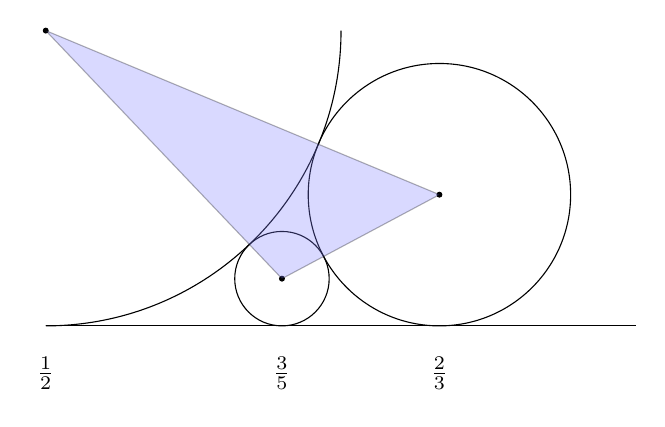
\begin{tikzpicture}[scale=30]
\draw (0.5,0)--(0.75,0);

\draw (3/5,1/5/5/2) circle (1/5/5/2);
\node at (3/5,-0.02) {$\frac{3}{5}$};
\draw[fill=black] (3/5,1/5/5/2) circle (0.001);

\draw (2/3,1/3/3/2) circle (1/3/3/2);
\node at (2/3,-0.02) {$\frac{2}{3}$};
\draw[fill=black] (2/3,1/3/3/2) circle (0.001);


\draw (1/2,0) arc (-90:0:1/2/2/2);
\node at (1/2,-0.02) {$\frac{1}{2}$};
\draw[fill=black] (1/2,1/2/2/2) circle (0.001);

\draw[fill=blue!50!white, opacity=0.3] (3/5,1/5/5/2)--(2/3,1/3/3/2)--(1/2,1/2/2/2)--cycle;
\end{tikzpicture}

\newpage  

\noindent Ford sells us his proof of Hurwitz's theorem with two good, heartening things:
\begin{quotation} \noindent
Our elementary proof proof will be free of continued fractions on the one hand and theory of the modular group on the other.
\end{quotation}
Is the theory of modular forms a ``scaffolding" for this more basic theory of circles?  Hurwitz's theorem states:
$$\# \left\{ \, \frac{p}{q} \in \mathbb{Q} : \left| \frac{p}{q} - \alpha \right| < \frac{1}{\sqrt{5} \, q^2 } \, \right\} =\infty \quad\text{ for }\quad \alpha \notin \mathbb{Q} $$
and $\sqrt{5}$ cannot be improved to any other number.\footnote{This is the beginning of the Markoff spectrum. The next number is $\sqrt{8}$. There is an excellent discussion by Carlos Matheus \texttt{https://matheuscmss.wordpress.com/2017/04/05/new-numbers-in-m-l/}.}  This could also be expressed as some of \textit{limit inferior}:
$$ \liminf_{n \to \infty}  n^2 \left| \xi - \frac{m}{n} \right| = \sqrt{5}$$
Ford states some results of continued fractions, that could be found in Khinchin's book (or newer sources) and finally he states a result for complex continued fractions - elements of $\mathbb{Q}(i)$ - which involve studying adjacent spheres.
$$\left| \frac{p}{q} - \alpha \right| < \frac{1}{\sqrt{3} \, q \overline{q}}$$
For complex numbers Hurwitz's theorem has $k = \sqrt{3}$ (and no elementary proof, as of 1938). \\  \\
It remains to prove the Hurwitz approximation result over $\mathbb{Q}$.  Ford's starting point is to equate each rational number with a vertical line. The circles it passes through are the rational approximations. \\
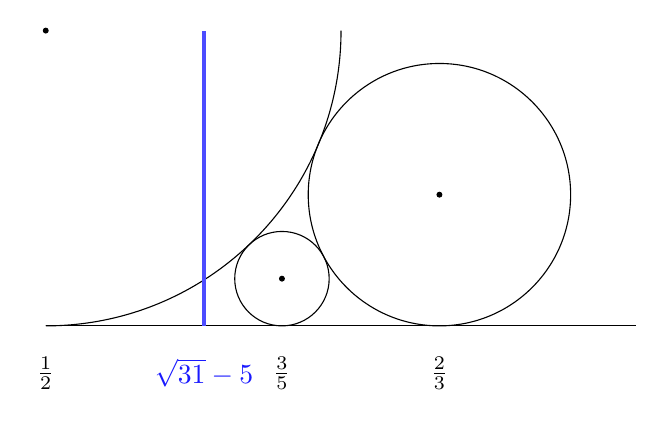
\begin{tikzpicture}[scale=30]
\draw (0.5,0)--(0.75,0);

\draw (3/5,1/5/5/2) circle (1/5/5/2);
\node at (3/5,-0.02) {$\frac{3}{5}$};
\draw[fill=black] (3/5,1/5/5/2) circle (0.001);

\draw (2/3,1/3/3/2) circle (1/3/3/2);
\node at (2/3,-0.02) {$\frac{2}{3}$};
\draw[fill=black] (2/3,1/3/3/2) circle (0.001);


\draw (1/2,0) arc (-90:0:1/2/2/2);
\node at (1/2,-0.02) {$\frac{1}{2}$};
\draw[fill=black] (1/2,1/2/2/2) circle (0.001);

%\draw[fill=blue!50!white, opacity=0.3] (3/5,1/5/5/2)--(2/3,1/3/3/2)--(1/2,1/2/2/2)--cycle;

\draw[blue!70!white, ultra thick] (0.567,0)--(0.567,1/8) ;
\node at (0.567,-0.02) {\color{blue!90!white}$\sqrt{31}-5$};

\end{tikzpicture} \\
Ford shows about a third of the time, you can get a very good approximation $k \geq \sqrt{5}$, and that this will happen infinitely often.  Later on the idea is that any \textit{diophantine approximation} result should have a cirlces proof or a continued fraction proof.  Or at least, the modular forms proof (once you find it) can always be simplified. \\ \\
By the way, this result fails for the {\color{yellow!50!black} golden ratio} $\xi = \frac{1+\sqrt{5}}{2}$, there are only finintely many fractions with $k > \sqrt{5}$.

\vfill
\begin{thebibliography}{}

\item Carlo Carminati,  Giulio Tiozzo (w/ Stefano Isola)\\
\textbf{Continued fractions with $\text{SL}(2, \mathbb{Z})$-branches: combinatorics and entropy} \texttt{arXiv:1312.6845} \\
\textbf{A canonical thickening of $\mathbb{Q}$ and the dynamics of continued fractions}
\hspace{1em}\texttt{arXiv:1004.3790}
\item Carlos Matheus, Carlos Gustavo Moreira \textbf{$HD(M∖L)<0.986927$} \texttt{arXiv:1708.06258}
\item Curtus T. McMullen \textbf{Uniformly Diophantine numbers in a fixed real quadratic field} \\ \texttt{https://doi.org/10.1112/S0010437X09004102}

\end{thebibliography}
\end{document}